%\documentclass[]{beamer}
%\documentclass[notes]{beamer}       % print frame + notes
%\documentclass[notes=only]{beamer}   % only notes
%\documentclass{beamer}              % only frames
\documentclass[handout]{beamer}
\usepackage{tikz}

\usepackage{algorithm2e}

\usetheme{Dresden}%%%%% developer's preference - may change based on preferences

%%%%%% UMass official color: https://www.umass.edu/brand/elements/color
\definecolor{UMassAmherst}{rgb}{0.533 0.11 0.11}
\usecolortheme[named=UMassAmherst]{structure}

\title{Combinatorias y Backtracking}
\author{MSc Edson Ticona Zegarra}
\institute{Campamento de Programaci\'on}
\date{}

%%%%%% obtained from: https://www.umass.edu/brand/elements/wordmarks-seal-and-spirit-marks
%%%%%% logos of other departments can also be obtained from the above link. Otherwise, consult your department website.

\begin{document}

\maketitle

\begin{frame}{Contenido}
\tableofcontents
\end{frame}

\section{Combinatoria}
\begin{frame}{Contenido}
\tableofcontents[currentsection]
\end{frame}

\begin{frame}{Combinatoria}
 \begin{itemize}
    \item Combinatoria es un \'area principalmente encargada del conteo de estructuras discretas
      \pause
    \item En la resoluci\'on de problemas, nos encontramos con diversas estructuras discretas
      \pause
    \item Contar la cantidad de estructuras posibles es b\'asico para la resoluci\'on de problemas
  \end{itemize}
\end{frame}

\begin{frame}{T\'ecnicas de conteo}
  \begin{itemize}
    \item Regla del producto: dadas $|A|$ posibilidades del conjunto $A$ y $|B|$ posibilidades del conjunto $B$, existen $|A|\times |B|$ maneras de combinar elementos de $A$ con $B$
      \pause
    \item Regla de la suma: dadas $|A|$ posibilidades del conjunto $A$ y $|B|$ posibilidades del conjunto $B$, existen $|A| + |B|$ maneras de que ocurran $A$ \textbf{o} $B$
      \pause
    \item Inclusion-Exclusion: es una generalizaci\'on de lo anterior cuando existen elementos en com\'un entre $A$ y $B$. $|A\cup B| = |A| + |B| - |A\cap B|$
  \end{itemize}
\end{frame}

\begin{frame}{T\'ecnicas de conteo}
  \begin{itemize}
    \item Strings: Dado un conjunto finito de posibles caracteres $S$, se puede obtener $|S|^k$ strings diferentes de longitud $k$
      \pause
    \item Subconjuntos: Cuantos subconjuntos se puede obtener de $n$ elementos: $2^n$
      \pause
    \item Permutaciones: De cuantas maneras se puede ordenar $n$ objetos sin repeticiones: $n!$
      \pause
    \item Combinaciones: De cuantas maneras se puede tomar $k$ elementos de $n$ posibles: $\binom{n}{k} = \frac{n!}{k!(n-k)!}$
  \end{itemize}
\end{frame}

\begin{frame}{Algoritmos de fuerza bruta}
  \begin{itemize}
    \item Un algoritmo de fuerza bruta es aquel que itera por todas las posibilidades, y analiza cada una de ellas
      \pause
    \item Entonces, todo algoritmo de fuerza bruta tendra complejidad proporcional a la cantidad de posibilidades multiplicado por el tiempo que demore en cada una de ellas
  \end{itemize}
\end{frame}

\section{Backtracking}
\begin{frame}{Contenido}
\tableofcontents[currentsection]
\end{frame}

\begin{frame}{Backtracking}
  \begin{itemize}
    \item Un algoritmo de backtracking analiza todas las soluciones \textit{viables}
      \pause
    \item La diferencia con un algoritmo de fuerza bruta es que analiza solo las soluciones viables, reduciendo el espacio de b\'usqueda
  \end{itemize}
\end{frame}

\begin{frame}{Backtracking}
  \begin{itemize}
    \item Primero se analiza la viabilidad de la soluci\'on dada
      \pause
    \item Luego se contruye el resto de soluciones, a partir de la actual
      \pause
    \item Finalmente se itera sobre cada una de la soluciones, analizando cada una de manera recursiva
  \end{itemize}
\end{frame}

\begin{frame}{El problema de las 8 reinas}
  \begin{definition}
    De cu\'antas formas se puede colocar 8 reinas en un tablero de ajedrez tal que ninguna de ellas amenace a otra
  \end{definition}
\end{frame}

\begin{frame}
  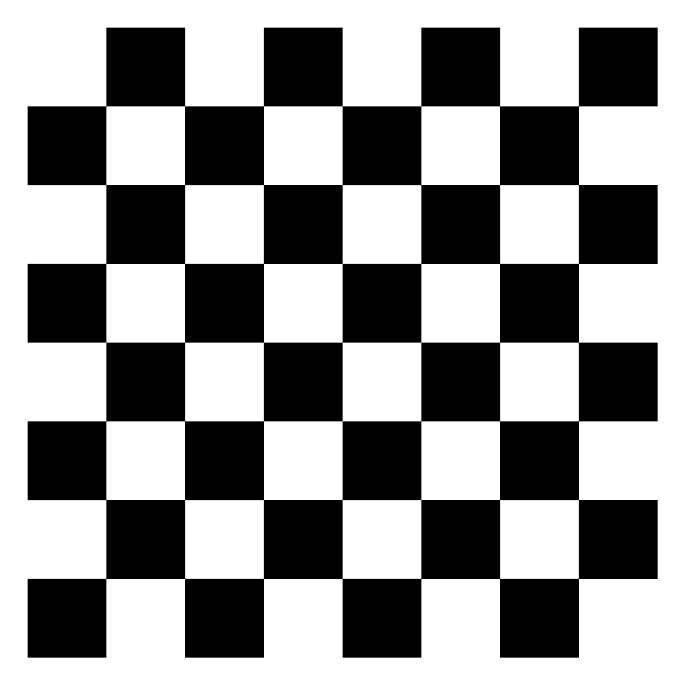
\begin{tikzpicture}[x=1cm]
    \foreach \y in {0,2,...,6}{
      \foreach \x in {0,2,...,6}{
        \fill (\x,\y) rectangle (1+\x,1+\y) rectangle (2+\x,2+\y);}}
  \end{tikzpicture}
\end{frame}

\end{document}
